\subsection{Sistema de Observabilidad en Operación}\label{subsec:resultado-c}

El tercer objetivo perseguía un sistema transversal de observabilidad estructurada capaz de diagnosticar el comportamiento del sistema en producción a través de componentes heterogéneos, soportado por infraestructura como código y notificaciones proactivas. El resultado obtenido es un subsistema operativo cuya evidencia abarca tanto los artefactos de telemetría como su impacto sobre la operación.

La telemetría estructurada en formato JSON se emite efectivamente desde los interceptores HTTP del \textit{frontend} (BFF en Nuxt) y del \textit{backend} (Go), con identificadores de correlación propagados a lo largo de la cadena de llamadas. La \autoref{fig:resultado-traza-correlacionada} ilustra la correlación extremo a extremo de una única acción de usuario que atraviesa el BFF, las funciones Lambda y una integración externa, identificada por un mismo \textit{correlation-id}.

\newcommand\resultadoTrazaCaption{Correlación extremo a extremo de una acción de usuario a través del BFF, las funciones Lambda y una integración externa. \hspace{1em}}
\begin{figure}[H]
  \centering
  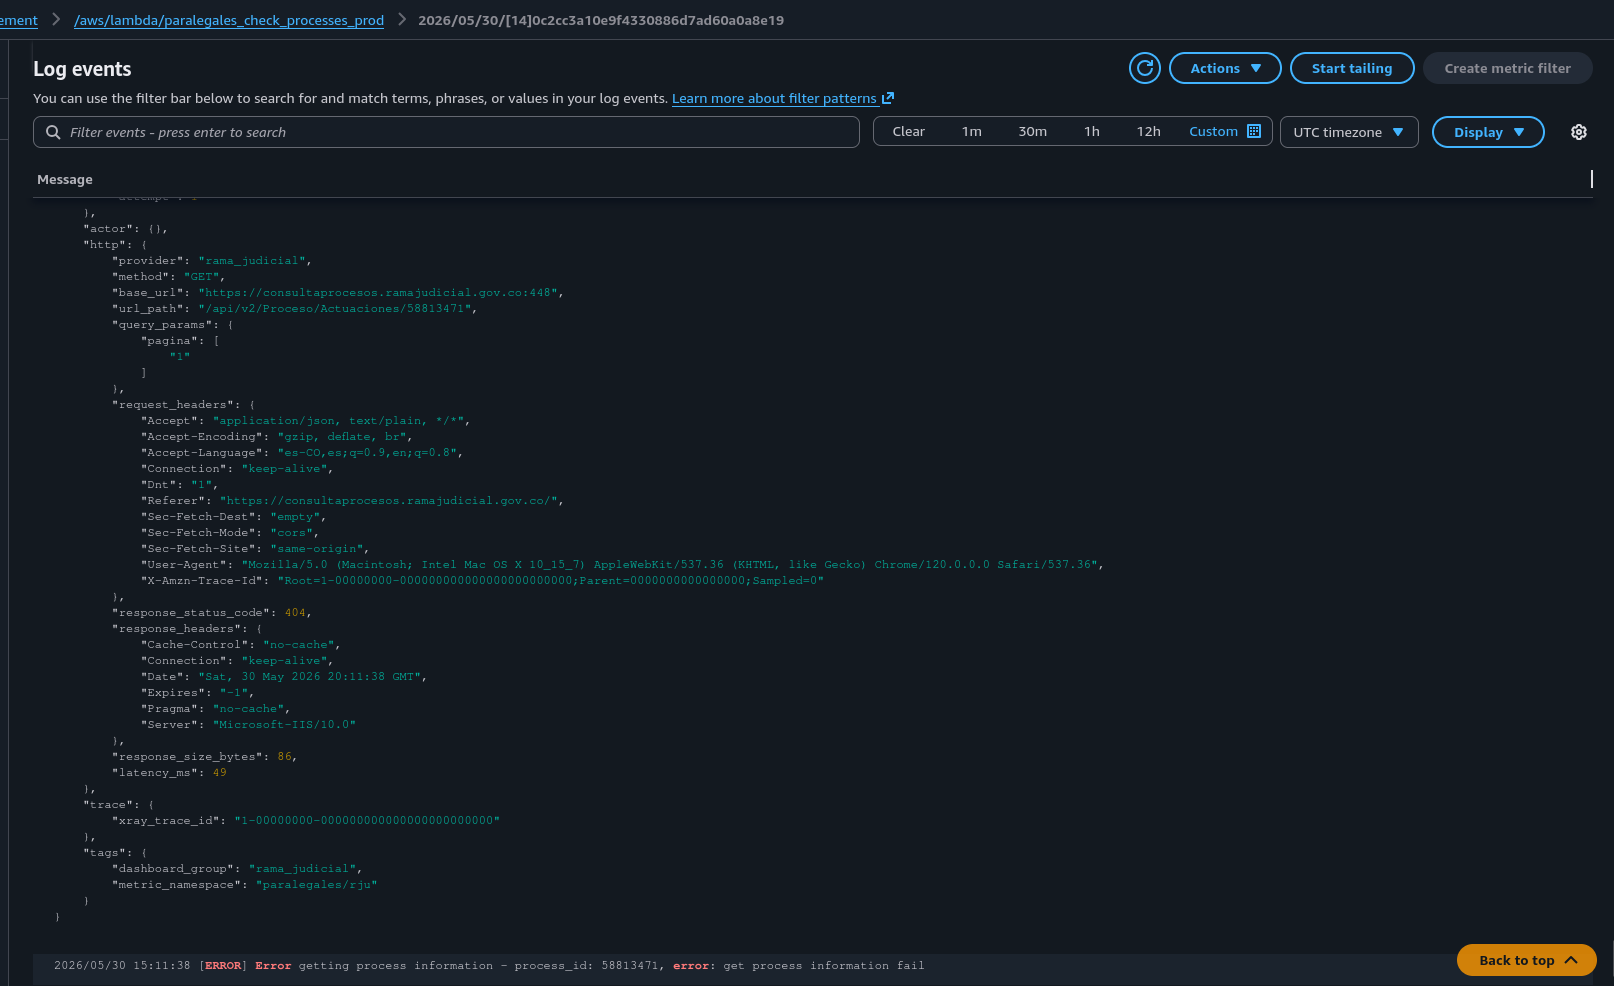
\includegraphics[width=1\textwidth]{img/figures/fig37-resultado-traza-correlacionada.png}
  \caption[\resultadoTrazaCaption]{\resultadoTrazaCaption Fuente: Elaboración propia.}
  \label{fig:resultado-traza-correlacionada}
\end{figure}

La infraestructura de observabilidad, definida y versionada como código mediante CloudFormation, se encuentra operativa: el panel de control de CloudWatch (\autoref{fig:dashboard-observabilidad}), las alarmas configuradas (\autoref{fig:dashboard-observabilidad-alerts}) y el canal de Telegram para notificaciones proactivas (\autoref{fig:telegram-alerts-observability}) funcionan de forma integrada.

El detalle de los indicadores que quedaron operativos se consigna en la \autoref{tab:sli-observabilidad}. Se trata de cinco métricas propias, derivadas de los \textit{logs} estructurados mediante filtros de métricas (\textit{metric filters}) y publicadas en el espacio de nombres \texttt{Paralegales/RJU}, todas dimensionadas por servicio a través de la clave \texttt{ServiceName}, junto con las dos compuertas de alerta configuradas sobre ellas.

\newcommand\sliObservabilidadCaption{Indicadores de nivel de servicio implementados sobre las integraciones externas, umbrales configurados y acciones asociadas. \hspace{1em}}

\begingroup
\renewcommand{\arraystretch}{1.3}
\begin{longtable}{|p{3.3cm}|p{3.4cm}|p{2.6cm}|p{1.8cm}|p{2.9cm}|}
  \hline
  \grayTableHeaderCell{3.3cm}{Indicador} &
  \grayTableHeaderCell{3.4cm}{Qué mide} &
  \grayTableHeaderCell{2.6cm}{Umbral configurado} &
  \grayTableHeaderCell{1.8cm}{Ventana} &
  \grayTableHeaderCell{2.9cm}{Acción disparada} \\
  \hline
  \endfirsthead

  \hline
  \grayTableHeaderCell{3.3cm}{Indicador} &
  \grayTableHeaderCell{3.4cm}{Qué mide} &
  \grayTableHeaderCell{2.6cm}{Umbral configurado} &
  \grayTableHeaderCell{1.8cm}{Ventana} &
  \grayTableHeaderCell{2.9cm}{Acción disparada} \\
  \hline
  \endhead

  \continuacionTablaFooter{5}
  \endfoot
  \endlastfoot

  \tableCell{\texttt{RJU\allowbreak RequestCount}} &
  \tableCell{Volumen de peticiones emitidas hacia el proveedor externo, por servicio.} &
  \tableCell{Sin umbral: indicador de contexto.} &
  \tableCell{No aplica} &
  \tableCell{Serie de tiempo en el panel de CloudWatch; línea base para interpretar la tasa de error.} \\
  \hline

  \tableCell{\texttt{RJU5xx\allowbreak Count}} &
  \tableCell{Respuestas con error de servidor (HTTP 5xx) devueltas por el proveedor externo, por servicio.} &
  \tableCell{Más de 10 errores, sumados sobre los ocho servicios.} &
  \tableCell{5 minutos} &
  \tableCell{Alarma \texttt{RJU-High5xx}: notificación al tópico SNS, que despacha a correo y a Telegram.} \\
  \hline

  \tableCell{\texttt{RJU4xx\allowbreak Count}} &
  \tableCell{Respuestas con error de cliente (HTTP 4xx), por servicio.} &
  \tableCell{Sin umbral: indicador de diagnóstico.} &
  \tableCell{No aplica} &
  \tableCell{Serie de tiempo en el panel; permite separar errores de uso de fallos del proveedor.} \\
  \hline

  \tableCell{\texttt{RJU\allowbreak LatencyMs}} &
  \tableCell{Latencia de respuesta del proveedor externo, en milisegundos, por servicio.} &
  \tableCell{Percentil 95 superior a 5000~ms en el peor de los servicios.} &
  \tableCell{5 minutos} &
  \tableCell{Alarma \texttt{RJU-\allowbreak High\allowbreak Latency}: notificación al tópico SNS, que despacha a correo y a Telegram.} \\
  \hline

  \tableCell{\texttt{RJU\allowbreak Status\allowbreak Distribution}} &
  \tableCell{Distribución de los códigos de estado HTTP, por servicio y por código.} &
  \tableCell{Sin umbral: indicador de diagnóstico.} &
  \tableCell{No aplica} &
  \tableCell{Consulta estructurada en el panel para el análisis de causa raíz.} \\
  \hline

  \caption[\sliObservabilidadCaption]{\sliObservabilidadCaption Fuente: Elaboración propia.}
  \label{tab:sli-observabilidad}
\end{longtable}
\endgroup

Las dos alarmas agregan la señal de los ocho servicios que consumen las APIs externas mediante expresiones de \textit{metric math}, de modo que la condición se evalúa sobre el comportamiento global de la integración y no sobre un servicio aislado. Ambas operan con un único periodo de evaluación de 300 segundos y tratan la ausencia de datos como estado no violatorio, para evitar alertas espurias en ventanas sin tráfico. Los umbrales no están fijados dentro de la definición de las alarmas sino declarados como parámetros de la plantilla de CloudFormation, con valores por defecto de 10 errores y 5000~ms, lo que permite ajustarlos por entorno sin modificar la definición de los recursos. Ambas alarmas notifican además el retorno al estado normal, de modo que el equipo recibe tanto el inicio como el cierre de cada episodio de degradación.

La consolidación de este subsistema produjo beneficios verificables sobre la operación de la plataforma. En primer lugar, dado que Paralegales consume APIs gubernamentales que históricamente presentan latencias altas o tiempos de inactividad, el sistema permite medir y auditar de forma objetiva la disponibilidad de dichos proveedores, separando de manera concluyente los fallos internos de las caídas en infraestructuras externas. En segundo lugar, al asociar de forma segura la actividad de red con los identificadores del usuario activo, como el ID de cuenta y el plan de suscripción, el equipo de soporte puede trazar e investigar el impacto de un error reportado por un cliente específico a través de toda la malla de microservicios. Finalmente, las alertas tempranas mediante mensajería instantánea permiten a los ingenieros mitigar fallos antes de que un porcentaje amplio de la base de usuarios perciba el impacto.

Conviene precisar, para cerrar, el estatus de estos resultados respecto del marco de \textit{Site Reliability Engineering} introducido en el marco conceptual \cite{Beyer2016}. Lo que el trabajo dejó operativo son los indicadores de nivel de servicio y las compuertas de alerta definidas sobre ellos, esto es, la instrumentación que vuelve medible el comportamiento de las integraciones críticas. Lo que no hizo fue formalizar objetivos sobre esos indicadores: los umbrales de la \autoref{tab:sli-observabilidad} son disparadores operativos de notificación, no SLOs declarados con un objetivo de cumplimiento en una ventana definida, y por sí solos no habilitan el cálculo de un \textit{error budget}. Los indicadores implementados son, no obstante, la condición previa para ello, dado que una vez acumulado un historial suficiente de estas series la definición de un objetivo y la derivación de su presupuesto de error constituyen un ejercicio de análisis sobre datos ya disponibles, sin necesidad de instrumentación adicional.

De ahí que tres elementos propios de la práctica de SRE queden explícitamente fuera de lo que este trabajo reporta: no se declararon SLOs, no se calcularon \textit{error budgets} y no se midió el MTTR. La limitación no es de diseño sino de disponibilidad de datos, pues los tres exigen un periodo de observación del sistema en producción y un registro sistemático de incidentes, con marcas de detección y de restablecimiento, que no estuvo disponible durante la pasantía, ya que el propio subsistema que produce esas series se puso en operación dentro de ella. Su definición constituye, por tanto, la continuación natural de este frente de trabajo: fijar objetivos de disponibilidad y de latencia sobre los indicadores de la \autoref{tab:sli-observabilidad}, instaurar un registro de incidentes que permita calcular el MTTR y emplear el presupuesto de error resultante como criterio para regular el ritmo de cambio de la plataforma.
